% Chapter 4

\chapter{Results}

\label{ch4}

In this section, we will perform DFT calculations with SIESTA with the intent to investigate functionalization in \textit{para}-\textit{para} NPG. Firstly, we will look into basic PP-NPG and its properties. Secondly, some calculations will be performed concerning individual dinitro-biphenyl molecules, which represent the bridges of the PP-NPG after functionalization with nitro groups. Finally, using the knowledge we acquired from the previous calculations, we explore the nitro-functionalized PP-NPG and the properties that will affect electron transport in this material.

\section{\textit{Para-para} NPG}
\textit{Para-para} connections in NPG present an special property, namely, the fact that both phenyls are able to be rotated through a central axis. It is known that phenyl-ring chains have trasport properties that depend on the torsional angle between the rings\parencite{Viljas2008}, which raises the question of what the effect of the torsional angle of the phenyl rings with respect to the 7-13-AGNR ribbon and with respect to one another might be, in terms of the inter-ribbon cross-talk. For this purpose, we study the electronic structure of PP-NPG.

Firstly, we obtained the relaxed structure up to a 0.01eV/\(\AA\) tolerance using the same parameters as for the basic NPG in section \ref{ele-npg}.
Equivalent and nonequivalent ribbons
% Pore orientation
%\subsection{Cross-talk}
Meaning\\
A measure of crosstalk \(\Delta E\) at \(\Gamma\)\\

\begin{figure}[h!]
	\centering
	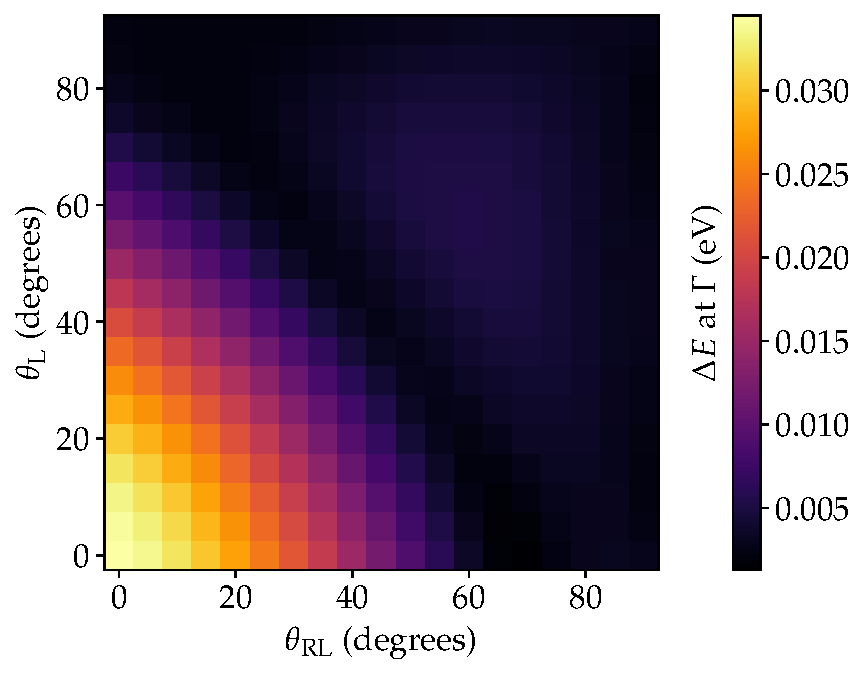
\includegraphics[width=0.7\linewidth]{Figures/2dmap}
	\decoRule
	\caption{2-dimensional plot of the band splitting of CB and CB+1 at the \(\Gamma\) point of PP-NPG.}
	\label{fig:2dmap}
\end{figure}


2D map. Decrease etc., 75\(^{\circ}\), from 3NN interaction in a TB picture?


\section{Dinitro-biphenyl molecule}
Properties (structure, (P)DOS...)\\
Molecular orbitals\\
Effect of the electric field (angle vs. \(\abs{\bm E}\), energy vs. angle...)

%----------------------------------------------------------------------------------------

\section{Dinitro-PP-NPG}
Resonance. Crosstalk

